Autotuning combined with various run-time adaptation,
genetic and machine learning techniques is a popular approach
in computer systems research to automatically explore multi-dimensional 
design and optimization spaces~\cite{atlas, europar97x, CGJ1997, Nis1998,
fftw, CSS99, VE00, KKO2000, FOK02, SAMP2003, Tapus:2002:AHT:762761.762771,
vista, spiral, LCYP04, la2004, FOTP2005, PE2006, HE2008, BCCP2008, JGVP2009,
Ansel:2009:PLC:1542476.1542481, Mars:2010:CAE:1772954.1772991,
DBLP:conf/cc/MooreC13, DBLP:conf/cf/ShenVSAS13, DBLP:conf/cgo/GreweWO13,
Miceli:2012:APA:2451764.2451792,
Manotas:2014:SSE:2568225.2568297,
ashouri2016cobayn}.

CK allows to unify such techniques by developing
a common, universal, portable, customizable, multi-dimensional
and multi-objective autotuning workflow as a CK module
(\textit{pipeline}%
\footnote{We use the term \textit{pipeline} similar to experiments in physics and electronics
where an output of one object is chained to an input of another one.}
from the public
\href{https://github.com/ctuning/ck-autotuning}{ck-autotuning} repository
with the \textit{autotune} function).
%
This allows us to abstract autotuning by decoupling it from the autotuned objects
such as \textit{"program"}.
%
Users just need to provide a compatible function \textit{"pipeline"} in a CK module 
which they want to be autotuned with a specific API including the following keys in both input and output:
\begin{itemize}

\item \textbf{dependencies} to describe software dependencies via portable package manager from the CK;

\item \textbf{choices} to expose various design and optimization knobs \textbf{c} such as algorithmic parameters, model topology, source-to-source transformations, compiler flags, hardware configurations, etc.;

\item \textbf{characteristics} to monitor optimized behavior \textbf{b} such as execution time, code size, compilation time, energy, memory usage, accuracy, resiliency, costs, etc.;

\item \textbf{features} to expose various object features \textbf{f} such as semantic program and data set features, hardware counters, platform properties, etc.;

\item \textbf{state} to define run-time system state \textbf{s} such as hardware frequencies, network status, cache state, etc.

\end{itemize}

   % === CK autotuning workflow ==================================================================
   %CK={"action":"prepare_for_latex", "cid":"slide:af4d04ba40b628dc", "file":"9a4de89400e0ff21-cropped.pdf", "path":"ck-assets", "ck_image":"yes", "ck_image_width":800}
   \begin{figure*}[!htbp]
     \centering
      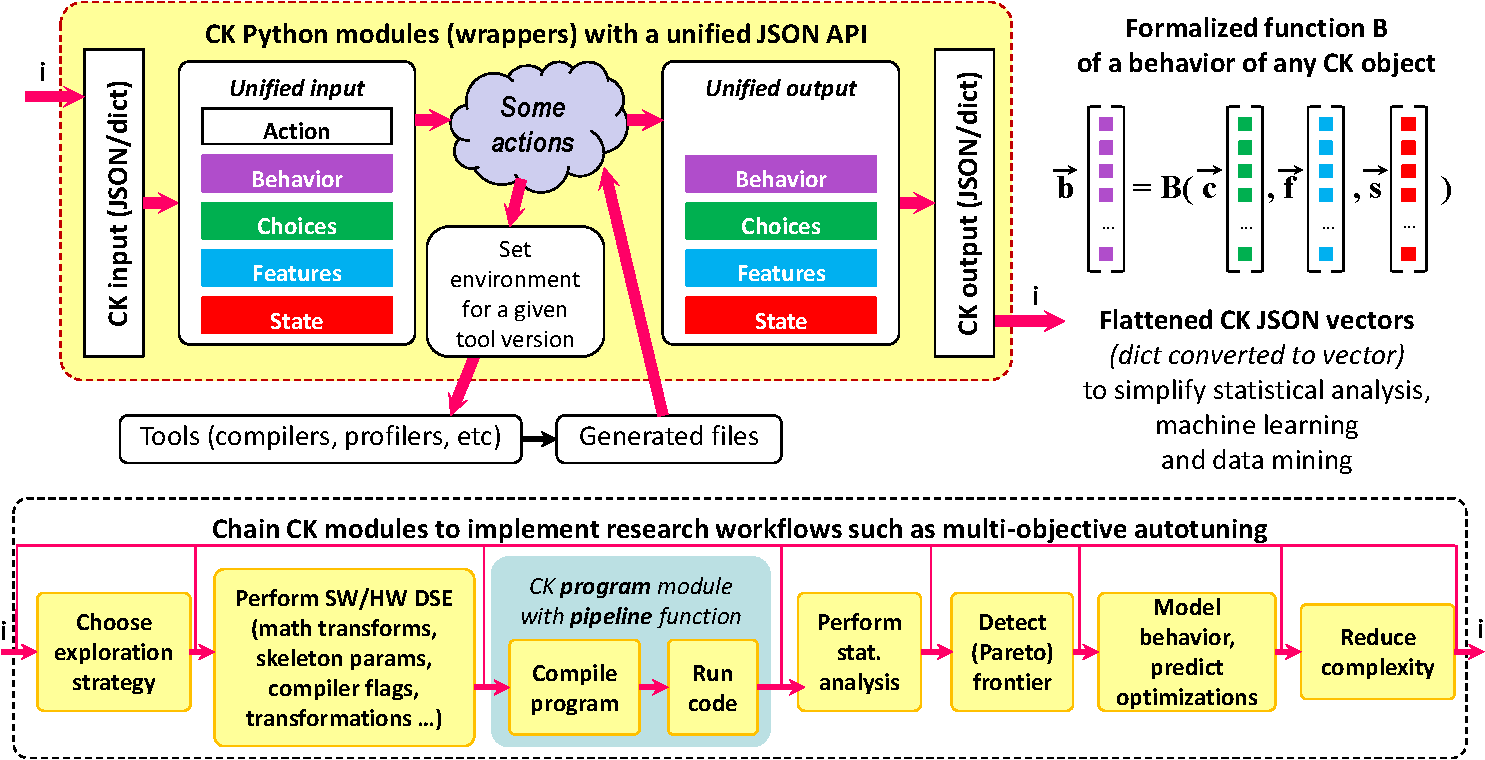
\includegraphics[width=6.6in]
      {ck-assets/9a4de89400e0ff21-cropped.pdf} %CK_URL={9a4de89400e0ff21-cropped.pdf}
     \caption{
       Chaining together various CK modules with JSON API and JSON meta information
       to implement universal, portable, customizable, multi-dimensional
       and multi-objective autotuner gradually extended by the community.
     }
     \label{fig:ck-universal-autotuning-workflow}
   \end{figure*}

Autotuning can now be implemented as a universal and extensible workflow
applied to any object with a matching JSON API by chaining together
related CK modules with various exploration strategies,
program transformation tools, compilers,
program compilation and execution pipeline, architecture simulators,
statistical analysis, Pareto frontier filter and other components,
as conceptually shown in Figure~\ref{fig:ck-universal-autotuning-workflow}.
%
Researchers can also use unified machine learning CK modules
(wrappers to R and scikit-learn~\cite{scikit-learn})
to model the relationship between \textbf{c}, \textbf{f}, \textbf{s}
and the observed behavior~\textbf{b}, increase coverage, speed up (focus) exploration,
and predict efficient optimizations~\cite{fursin:hal-01054763,cm:29db2248aba45e59:cd11e3a188574d80}.
%
They can also take advantage of a universal complexity reduction module
which can automatically simplify found solutions without changing their behavior,
reduce models and features without sacrificing accuracy,
localize performance issues via differential analysis~\cite{FOTP04},
reduce programs to localize bugs, and so on.

Even more importantly, our concept of a universal autotuning workflow,
knowledge sharing and artifact reuse can help teach students
how to apply a well-established holistic and top-down
experimental methodology from natural sciences to continuously 
learn and improve the behavior of complex computer systems~\cite{ck-date16,fursin:hal-01054763}.
%
Researchers can continue exposing more design and optimization knobs~\textbf{c},
behavioral characteristics~\textbf{b}, static and dynamic features~\textbf{f},
and run-time state \textit{state} to optimize and model behavior
of various interconnected objects from the workflow depending on their
research interests and autotuning scenarios.

Such scenarios are also implemented as CK modules
and describe which sets of choices to select, 
how to autotune them and which multiple characteristics to trade off.
%
For example, existing scenarios include
"autotuning OpenCL parameters to improve execution time",
"autotuning GCC flags to balance execution time and code size",
"autotune LLVM flags to reduce execution time",
"automatically fuzzing compilers to detect bugs",
"exploring CPU and GPU frequency in terms of execution time and power consumption",
"autotuning deep learning algorithms in terms of speed, accuracy, energy, memory usage and costs",
and so on.

You can see some of the autotuning scenarios using the following commands:\newline
\begin{flushleft}
\texttt{\$ ck pull repo:ck-crowdtuning}\newline
\texttt{\$ ck search module --tags="program optimization"}\newline
\texttt{\$ ck list program}\newline
\end{flushleft}
%
They can then be invoked from the command line as follows:\newline
\begin{flushleft}
\texttt{\$ ck autotune program:[CK program alias] --scenario=[above CK scenario alias]}
\end{flushleft}
